\chapter{Minecraft as a MicroPsi 2 World}
\label{chap:4}
The objective of this project is to build and test an interface in between MicroPsi and Minecraft, so that a Minecraft world can be used as a simulation environment for experiments within the MicroPsi framework, which will act as an artificial player. Since there exist open source projects that perform many of the tasks required for this goal, \texttt{Spock}, the Python Minecraft bot framework by Nick Gamberini, and \texttt{Minecraft}, the Python Minecraft clone by Michael Fogleman, have been chosen as foundations that have been implemented into the MicroPsi framework. \texttt{Spock} facilitates communication with Minecraft servers. To make the new simulation environment monitorable, \texttt{Minecraft} by Fogleman has been used to implement a 3D visualisation of the Minecraft world in the web interface. The following section gives an overview of the implemented modules.

\section{Overview}

%TODO !!! Herr Wirsing wird diesen Teil genau anschauen. Es braucht ein ordentliches UML Diagramm und eine gute Erklärung!

%TODO !!!!! Zu deiner eigenen Arbeit vermisse ich echte UML Diagramme. Herr Wirsing wird dich sicher nach der Architektur fragen, deswegen bereite dich darauf vor. Außerdem passt dein Text im Moment nicht zu deinem “Architektur”-Diagramm. Kapitel 4.1 wird für Herrn Wirsing DAS Kapitel. Deswegen muss das wirklich gut sein, nicht zu implementierungsnah, sondern eher aus Sicht der Architektur. Der Zusammenhang zwischen MicroPSI und Minecraft muss klar werden, ebenso dein Beitrag und die generelle Idee der Implementierung.

The modular architecture of MicroPsi allows it to add new simulation environments (or worlds, as they are called in MicroPsi) fairly easily. To communicate with a MicroPsi node net, a world needs an interface, which is called \emph{world adapter}, as it is described in section~\ref{sec:2:MicroPsi}. Looking at the Minecraft side, communication with a Minecraft server typically requires a constant flow of data packets going in and out, as it is described in section~\ref{sec:3:relatedprojects}. To add a Minecraft world to MicroPsi, the demands of both sides have to be met.

%TODO So richtig verstehe ich nicht, wo MicroPsi reinspielt...

The contributions of this project are divided into the four modules \texttt{MinecraftWorld}, \texttt{MinecraftWorldadapter}, \texttt{MinecraftClient} and \texttt{MinecraftVisualisation}. The resulting architecture is displayed in figure~\ref{uml_mc}. The \texttt{MinecraftClient} manages the communication with the Minecraft server, provides convenient functions and data structures for sending and responding to packets and stores and regularly updates a simple representation of the environment data it receives from the server. The \texttt{MinecraftVisualisation} module generates 3D images that display the current state of the Minecraft environment, based on the world data it receives from the \texttt{MinecraftClient}. The \texttt{MinecraftWorldadapter} represents the interface towards the MicroPsi node net. It defines the \emph{data sources} that are filled with data from the \texttt{MinecraftClient} and accessed by the node net. It furthermore defines the \emph{data targets} that, conversely, are filled by the node net and translated to actions that the \texttt{MinecraftClient} executes. What ties it all together is the \texttt{MinecraftWorld} module. It provides a step function that is called frequently by the world runner and that advances the \texttt{MinecraftClient}, the \texttt{MinecraftWorldadapter} and the \texttt{MinecraftVisualisation}.

%TODO Das ist kein UML

\begin{figure}[h]
  \centering
    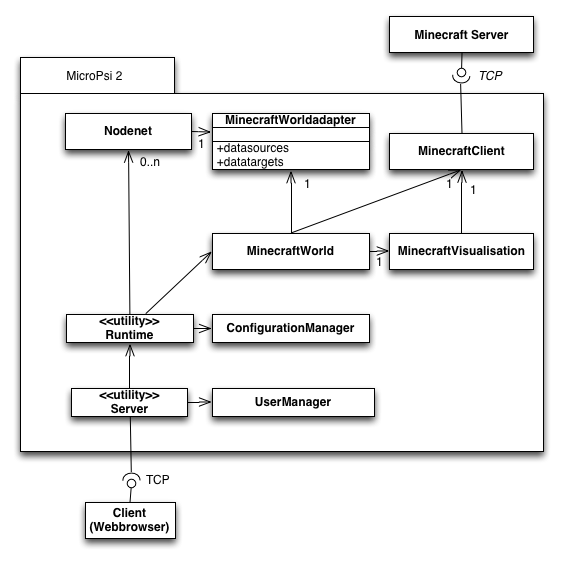
\includegraphics[width=11cm]{graphics/UML_MicroPsi_mit_spock_v14}
  \caption{The architecture of MicroPsi with the new Minecraft interface}
  \label{uml_mc}
\end{figure}

The \texttt{MinecraftVisualisation} module can be exchanged or cut off completely very easily, as no other modules depend on it. Instead of the visualisation, a placeholder image can be displayed in the web interface, which does not effect the functionality of the simulation. The \texttt{MinecraftVisualisation} module itself depends on the data structures of the \texttt{MinecraftClient}, though. This means, exchanging the \texttt{MinecraftClient} would require adjustments of the \texttt{MinecraftVisualisation}, to still function as intended. The same holds true for the \emph{data sources} and \emph{targets} in the \texttt{MinecraftWorldadapter}.

    \section{Using \texttt{Spock} as the \texttt{MinecraftClient}}

As mentioned above, the purpose of the \texttt{MinecraftClient} is to manage the communication with the Minecraft server and to provide a representation of the agent's environment. The calculation of the simulation environment, does not take place in MicroPsi itself, but on a regular Minecraft Server. Instead, \texttt{Spock} is integrated into MicroPsi and represents the simulation world towards it. \texttt{Spock} (in the following the \texttt{MinecraftClient}) communicates with the Minecraft server via the \emph{client server protocol} and provides data that can be used as \emph{data sources} for the world adapter and translates the data from the \emph{data targets} to actions in the simulation environment. That way, to MicroPsi it looks like the \texttt{MinecraftClient} is the simulation environment itself, where, in fact, it is the interface to the game world server.

%%TODO event loop handling frequency bs

The original event loop of the bot framework had to be dissolved and rebuilt as an \texttt{advanceClient} function that is called as a part of the \texttt{MinecraftWorld}'s step function. For every invocation of the \texttt{advanceClient()} function the \texttt{MinecraftClient} sends its packet queue to the server through a TCP socket, receives incoming packets from the server, dispatches the received packages appropriately and, if necessary, prepares the necessary actions that it is instructed to by the \texttt{MinecraftWorldadapter}'s \emph{data targets}~(see figure~\ref{spock_loop}).

\begin{figure}[h]
  \centering
    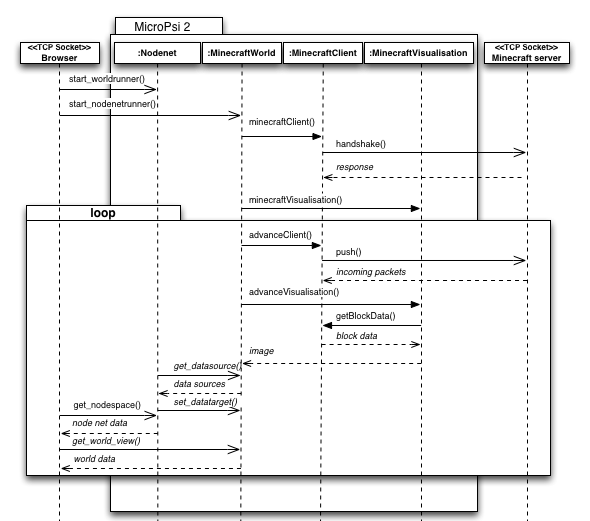
\includegraphics[width=15cm]{graphics/sequencediagram_v14}
  \caption{A simplified sequence diagram of the flow of data in between the web browser, MicroPsi and a Minecraft server in respect to the contributions of this thesis}
  \label{spock_loop}
\end{figure}

Subsequently, a system for translating \emph{data targets} to actions had to be implemented. In most cases, performing actions means to let the \texttt{MinecraftClient} send a particular set of packets to the Minecraft server. For this purpose, the class \texttt{PsiDispatcher} has been added to the \texttt{MinecraftClient}, which is described in section~\ref{extensions_client}.


        \subsection{Overview of the \texttt{MinecraftClient}}
The \texttt{MinecraftClient} holds all the functionalities that enable it to act as an artificial Minecraft player. It implements the packet based \emph{client server protocol} and uses it to communicate with Minecraft servers. It provides data structures that reflect the concepts of a Minecraft world and uses these to store the data it receives from the server. It is heavily based on \texttt{Spock}, which has been developed as an educational project. The scope of the original project was to build a pure Python Minecraft bot framework without dependencies. This has been achieved with one minor exception: if one would like to connect the bot to an official Minecraft online server, the packets have to be encrypted using the Python cryptography library PyCrypto. It consists of several classes, which are outlined in figure~\ref{spock_UML}.

%TODO remove world from variables. in uml

\begin{figure}[h]
  \centering
    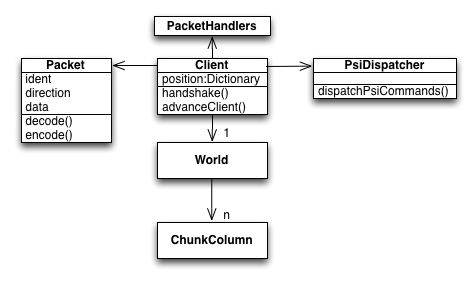
\includegraphics[width=12cm]{graphics/spockUML_v14}
  \caption{The most important classes of the \texttt{MinecraftClient}}
  \label{spock_UML}
\end{figure}

The main class \texttt{Client} provides the internal logic that is necessary to implement communication with Minecraft servers. Most importantly, these are the function handshake(), which initiates the communication with the server by performing the actions of the \emph{login sequence}\footnote{\url{http://wiki.vg/Protocol_FAQ}} and the function advanceClient() that performs one iteration of the client's lifecycle.


The class \texttt{Client} furthermore holds a reference to an instance of the class \texttt{World} and uses instances of the classes \texttt{Packet} to implement the \emph{client server protocol}. The class \texttt{World} holds the internal representation of the gameworld. It brings functions, data structures and classes that represent single sections of the environment (such as \texttt{ChunkColumn}s) to represent the gameworld and to obtain information about what block sits where. \texttt{ChunkColumn}s manage dictionaries that store chunk data as integers.

Instances of the class \texttt{Packet} represent single packets of the \emph{client server protocol} as they are described in section~\ref{client_server_protocol}. They bring functions to encode and decode packet data to get to the payload or to be able to send packets to the Server.

The collection of classes \texttt{PacketHandlers} registers one handler class for each packet type that the client is supposed to deal with by default. For every iteration of the \texttt{advanceClient()} function incoming packets are dispatched to these handlers. Figure~\ref{packet_handling} gives an example.


		\begin{figure}[ht]
			\centering
			\begin{minipage}{11cm}
				\begin{pseudocode}
#Chunk Data - Update client World state
@phandle(0x33)
class handle33(BaseHandle):
	@classmethod
	def ToClient(self, client, packet):
		client.world.unpack_column(packet)
					\end{pseudocode}
				\caption{By default, this function handles "Chunk Data (0x33) packets.}
				\label{packet_handling}
			\end{minipage}
		\end{figure}

        \subsection{Extensions to the \texttt{MinecraftClient}}
        \label{extensions_client}
To function as a simulation world for MicroPsi, the \texttt{MinecraftClient} has to translate activation of the \emph{data targets} in the \texttt{MinecraftWorldadapter} to actions. Therefore, a reference to the new class \texttt{PsiDispatcher} has been added to the \texttt{MinecraftClient} that holds a single function \texttt{dispatchPsiCommands()}. Its purpose is to check the values of the \emph{data targets} frequently and invoke appropriate actions, if necessary. The \texttt{PsiDispatcher} is called as a part of the \texttt{advanceClient} function. It checks each available data target, and if necessary invokes an appropriate action (eg. sending a packet). The following listing gives an example for a data target that has been specified to indicate that the agent is supposed to move one block towards the direction of the x-axis.

		\begin{figure}[ht]
			\centering
			\begin{minipage}{11cm}
				\begin{pseudocode}
#check for MicroPsi input
if self.client.move_x > 0:
    self.client.push(Packet(ident = 0x0B, data = {
        'x': self.client.position['x'] + 1,
        'y': self.client.position['y'],
        'z': self.client.position['z']
        'on_ground': False,
        'stance': self.client.position['y'] + 0.11
        }))
					\end{pseudocode}
				\caption{The \texttt{PsiDispatcher} checking for activation of the move-x data target and invoking the according action by sending a ``Player Position'' packet}
				\label{listing_dispatch}
			\end{minipage}
		\end{figure}

    \section{Module \texttt{MinecraftVisualisation}}

%TODO Wo ist die zu sehen? (Minecraft world step function) 
    
Another important part of this project is the visualisation component. There are two main reasons for its realisation. The first reason is that the agent's behaviour within the simulation environment is supposed to be visually monitored from the MicroPsi web interface---in a both efficient and pleasurable manner. The second reason is that the image data is supposed to be processed by the node net as a data source itself in the future. The module contains classes and functions that provide an interface to the OpenGL context that generates the 3D graphics. This section gives an overview about what data the visualisation uses to generate images of the environment. 

Inside the \texttt{MinecraftWorld}'s step function, the visualisation module is called to generate a 3D model of the Minecraft world and the agent within. The visualisation component reads from the \texttt{MinecraftClient}'s internal gameworld representation to generate the 3D model. This means that, from pure Minecraft world data, a 3D visualisation is generated. It is supposed to display a bird's-eye view of the current chunk to give a good overview of the bots environment and forward it to the web interface.

\begin{figure}[h]
  \centering
    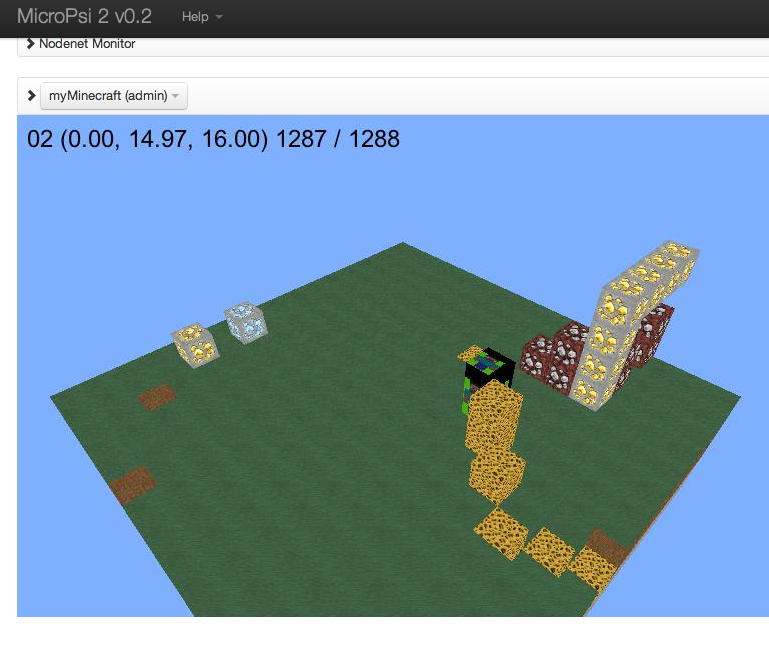
\includegraphics[width=10cm]{graphics/visualisation_screen}
  \caption{An image generated by the \texttt{MinecraftVisualisation} component}
  \label{vis_screen}
\end{figure}

Specifically, the representation of the chunk, the agent is located in, is fetched and for each solid cube in this chunk, a corresponding cube is rendered within the visualisation using Pyglet's OpenGL abstraction~(see figure~\ref{vis_screen}). Each block has textures matching its type. The implemented format for the textures is compatible to the widely available Minecraft texture packs. That way, the visualisation's look can be changed completely within seconds. The resulting images are exported as PNG files which are stored in memory and which are delivered to the web interface which is requesting them frequently. A refresh rate of six or more images per second creates the impression of a video stream.

The resulting architecture can be described as an implementation of a \emph{model-view-controller} pattern (see figure~\ref{mvc}). Therefore the \texttt{MinecraftWorld} acts as the \emph{controller} that iterates through the life cycles of both the \texttt{MinecraftClient} and the \texttt{MinecraftVisualisation}. Everytime the visualisation component that resembles the \emph{view} updates the 3D view, it fetches the required world data from the \texttt{MinecraftClient}, which acts as the \emph{model}.

\begin{figure}[h]
  \centering
    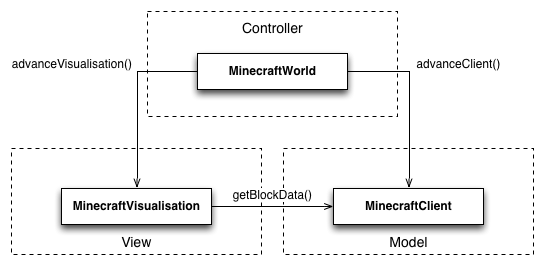
\includegraphics[width=12cm]{graphics/mvc}
  \caption{The model-view-controller pattern used for the visualisation module}
  \label{mvc}
\end{figure}

    \section{Module \texttt{MinecraftWorldadapter}}

%TODO Wozu ist diese Klasse da? Ist das eine spezielle Implementierung?

The \texttt{MinecraftWorldadapter} provides the necessary interfaces that let a \texttt{MinecraftClient} be controlled by a MicroPsi node net. Most importantly, these are the before mentioned \emph{data sources} and \emph{targets}. It inherits mutator methods for these from its parent class \texttt{WorldAdapter}, which itself inherits from \texttt{WorldObject}, which is the superclass of all agents and world objects, as they are described in section~\ref{microPsiWorld}. As it holds a reference to the according \texttt{MinecraftClient}, it has full access to the environment data and other properties of the client. This allows it, to easily implement simple ``sensors'' by developing algorithms that utilise and search the provided data structures. An example is given in the following section.
    
    \section{Case Study}
    \label{case_study}
    
%TODO Das Ziel der Case Study hab ich leider auch sehr spät verstanden. Hier muss auch noch etwas Arbeit rein.

%TODO beginne mit einer Szenario Beschreibung!

%TODO connected? Wirklich verbunden?

To explain, how the new interface can be utilised, we will construct a simple case study in the following. As it only consists of a primitive wiring between sensors and actuators, the scientific value in terms of AI research is low. However, it shall suffice as a proof of concept that the interface is functional and may serve as a foundation for future experiments.

The scenario consists of a single agent that is placed in a Minecraft world. It is standing on a flat surface that is made out of \emph{grass} blocks. Next, a block of \emph{diamond} is placed in the same chunk. The agent is supposed to automatically approach this block, depending on where it has been placed. Therefore it is controlled by a MicroPsi node net, which is set up as described in the following.

\paragraph{Node net}$\;$ \\

After the web interface has been started, a new node net is generated. Inside it, four sensor nodes have been created. These nodes shall represent sensors, that can detect if a block of diamond can be located in a particular cardinal direction. Furthermore, four actuator nodes are created, that represent the agent's movements towards each of the same four directions. Next, four links are generated that in the following forward activation from the sensor nodes to the actuator nodes that make the agent move towards the according direction. Finally, an activator node is added, that defines the general ability of links in this particular node net to forward activity. The resulting node net is displayed in figure~\ref{nodenet_setup}.

\begin{figure}[h]
  \centering
    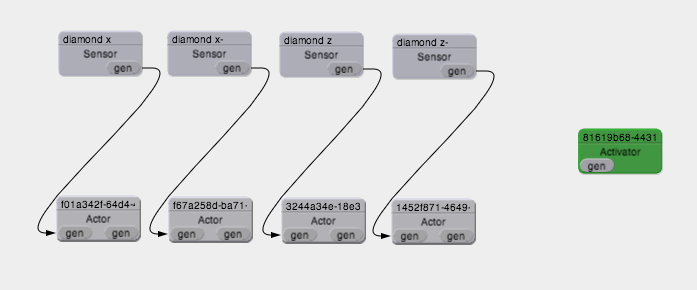
\includegraphics[width=14cm]{graphics/nodenet_setup}
  \caption{The node net set up for this experiment}
  \label{nodenet_setup}
\end{figure}

\paragraph{Data sources}$\;$ \\

To implement the before mentioned sensors, suitable algorithms have to be integrated into the \texttt{MinecraftWorldadapter}. For sensors that detect \emph{diamond} blocks in the current chunk, this could be realised by fetching the chunk data and examine it for the according block type. If a block is found, its coordinates are modified it respect of the agent's own position to express the sensor values. A possible implementation is outlined in figure~\ref{listing_sensors}. 


		\begin{figure}[ht]
			\centering
			\begin{minipage}{17cm}
				\begin{pseudocode}
for y in range(0, 16):
 current_section = current_column.chunks[int((bot_block[1] + y -  2) / 16)]
 if current_section != None:
  for x in range(0, 16):
   for z in range(0, 16):
    current_block = current_section['block_data'].get(x, _block[1] + y - 10 / 2)), z)
    if current_block == 56: #Diamond Ore
     diamond_coords = (x + x_chunk * 16,y,z + z_chunk * 16)
     self.datasources['diamond_offset_x'] = bot_block[0] - coords[0] - 2
     self.datasources['diamond_offset_z'] = bot_block[2] - coords[2] - 2
     self.datasources['diamond_offset_x_'] = (bot_block[0] - coords[0]) * -1 - 2
     self.datasources['diamond_offset_z_'] = (bot_block[2] - coords[2]) * -1 - 2
			\end{pseudocode}
		\caption{Searching the current section for a diamond block and, if it is found, filling the concerning data sources with the distance towards it.}
		\label{listing_sensors}
	\end{minipage}
\end{figure}

Next, in the node net editor the four sensor node are edited in such way, that they are associated with the new \emph{data sources}. For every iteration, the node net now will update the sensor values with the values calculated for the \emph{data sources} of the \texttt{MinecraftWorldadapter}.

\paragraph{Data targets}$\;$ \\

Subsequently, data targets have to be defined, that represent the actuators for moving forwards, backwards, left and right. Moreover, suitable methods have to be integrated into the \texttt{PsiDispatcher}. The example from section~\ref{extensions_client} illustrates just this. Equally, in the node net editor the actuator nodes have to be associated with the new \emph{data targets}.

\paragraph{Execution}$\;$ \\

To conclude the experiment, a chunk in a Minecraft world is set up that way, that it contains only a plane, without other obstacles, that the agent might move around on freely, as well as a diamond block that is placed at its center. 

%TODO verstehe ich nicht

Then, the agent is placed in one of the chunk`s corners. We furthermore define that the activation of the sensors equals the distance to the diamond block in the regarding direction. The data sources get filled through searching in the entire section, as figure~\ref{listing_sensors} displays.
    
%TODO ich habe node nets immer noch nicht verstanden. Das wäre hier sehr wichtig!

%TODO Was ist hier die Aufgabe von MicroPsi? Warum braucht man es im Hintergrund überhaupt? Ist das hier nicht nur eine einfache Reaktion auf Semsorwerte?
    
In every step of the world, the client will check the data targets and therefore move towards the diamond. Once it gets to a distance towards the diamond, that is below a defined threshold, the sensors will stop sending activation, and the agent will stop moving towards it. Note that if the node net runner and the world runner run asynchronously, there might be a delay in the shift of behaviour of the agent. Hence, it is advised, to run them synchronously or at least with a timing close to each other.



If we start a simulation like this, the nodes of the sensors that point to the diamond light up green and their activation is forwarded to the actuators. The bot moves towards the diamond until it is closer than the sensor's threshold, to not detect the diamond anymore---for this experiment the threshold has been set to two blocks. Then it stops moving~(see figure \ref{diamond_screens}).

\begin{figure}[h]
  \centering
    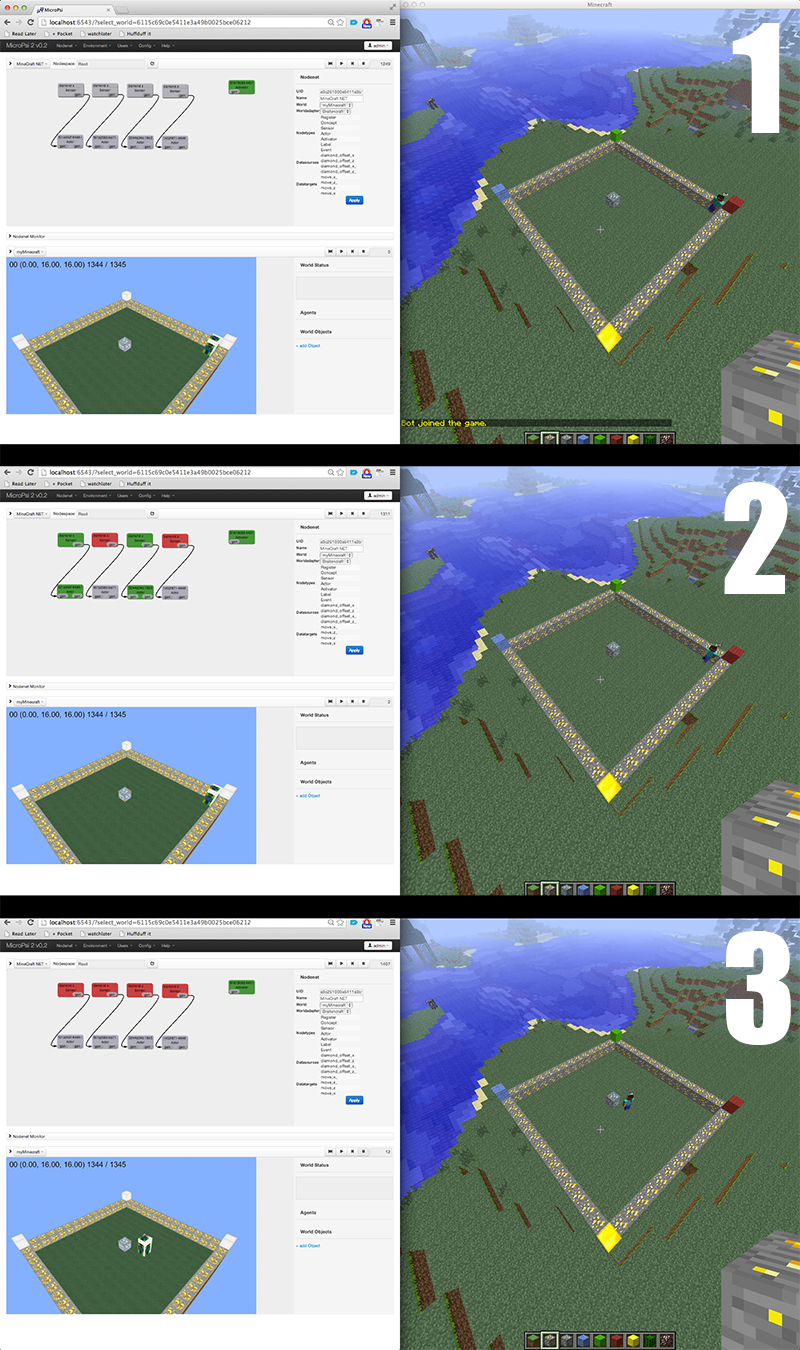
\includegraphics[width=10cm]{graphics/diamond_screens}
  \caption{1. Neither node net, nor agent show any activity, as the experiment did not start yet.  2. The sensors that indicate a diamond towards the negative x- and z-axes light up green---so do the according actuators. The agent starts moving.  3. The agent arrived close enough to the diamond, that the sensors stop forwarding activation. The agent stops moving.}
  \label{diamond_screens}
\end{figure}

        \subsection{Evaluation}
        
%TODO Für die Evaluation ist interssant, ob das Interface funktioniert, wie gut es funktioniert (Geschwindigkeiten etc.), ob es einfach zu bedienen ist....
        
Now, that a proof-of-concept experiment has been concluded, the implementation can be evaluated.
The experiment obviously shows that an interface in between a Minecraft world and the MicroPsi framework has been implemented. In the experiment, the agent concludes the appropriate action, if a node net actuator node receives activation and stops doing so, when it stops receiving activation.

With MicroPsi node nets in the back, more complex experiments can now be thought of and implemented, that lead to more complex behaviours of the agent.

An issue that remains concerning is that the reaction time in between changes in the node net and the according changes of the agent's behaviour seems to be too long, for differing timing of the node net runner and the world runner.

This issue could be resolved, by making the bot faster---for example, by sending the visualisation image data directly to the web interface, without writing it to the hard disk first.

    \section{Summary}
This chapter presented the implementation of the Minecraft interface for MicroPsi, which consists of the modules \texttt{MinecraftClient}, \texttt{MinecraftVisualisation} and \texttt{MinecraftWorld}. The \texttt{MinecraftClient} facilitates the communication with the Minecraft server; the \texttt{MinecraftVisualisation} delivers OpenGL rendered image data of the environment and the \texttt{MinecraftWorld} serves as the actual world adapter in between the \texttt{MinecraftClient} and MicroPsi.
Next, a case study has been performed and evaluated. A MicroPsi client had to move towards a block of a particular type. It showed that the interface is functional and ready for more sophisticated experiments.
With the implementation of the interface and the following proof-of-concept case study the scope of this thesis has been completed. The last chapter contains a summary and an outlook towards future applications.